\documentclass[14pt]{extarticle}

\usepackage{geometry}
\usepackage{amsmath,amsthm,amssymb}
\usepackage[utf8]{inputenc}
\usepackage[T1,T2A]{fontenc}
\usepackage{bold-extra}
\usepackage[english,russian]{babel}
\usepackage{indentfirst}
\usepackage{graphicx}
\graphicspath{ {images/} }
\usepackage{float}
\usepackage{listings}
\usepackage{lmodern}
\usepackage{appendix}
\usepackage{braket}
\usepackage{cite}
\usepackage[nottoc,numbib]{tocbibind}

\geometry{
a4paper,
left = 20mm,
right = 15mm,
bottom = 20mm,
top = 20mm,
}
\renewcommand{\rmdefault}{ftm} % TimesNewRoman
\renewcommand{\baselinestretch}{1.5} 

\begin{document}

\begin{titlepage}
	\begin{center}
		\small{ФЕДЕРАЛЬНОЕ ГОСУДАРСТВЕННОЕ БЮДЖЕТНОЕ ОБРАЗОВАТЕЛЬНОЕ}\\ 
			УЧРЕЖДЕНИЕ ВЫСШЕГО ОБРАЗОВАНИЯ\\
			«МОСКОВСКИЙ ГОСУДАРСТВЕННЫЙ УНИВЕРСИТЕТ\\
			имени М.В.ЛОМОНОСОВА»\\
		\hfill \break
		ФАКУЛЬТЕТ ВЫЧИСЛИТЕЛЬНОЙ МАТЕМАТИКИ И КИБЕРНЕТИКИ\\
		КАФЕДРА СУПЕРКОМПЬЮТЕРОВ И КВАНТОВОЙ ИНФОРМАТИКИ\\
		\vfill
		ЗАДАНИЕ 2 \\
		\textbf{<<ПАРАЛЛЕЛЬНАЯ СОРТИРОВКА БЭТЧЕРА>>}\\
		КУРСА \\
		\textbf{<<ПАРАЛЛЕЛЬНЫЕ ВЫЧИСЛЕНИЯ>>}\\
	\end{center}	
	\vfill
	\begin{flushright}
		Выполнил студент группы м118:\\
		Пухов Д. Н.\\
		Дата подачи: 28.02.2018
		\vfill
	\end{flushright}
	
	
	\begin{center}
		Москва \\
		2018
	\end{center}
	
	\thispagestyle{empty}

\end{titlepage}

\tableofcontents
\newpage



\section{Формулировка задачи}
Дана регулярная прямоугольная сетка, узлы которой определяются следующей структурой:
\begin{lstlisting}
struct Point
{
	float coord[2];
	int index;
} P[n1*n2];
\end{lstlisting}
Точки данной сетки имеют координаты
\begin{lstlisting}
P[i*n2+j].coord[0] = x(i,j)
P[i*n2+j].coord[1] = y(i,j)
\end{lstlisting}
Индекс определяется так:
\begin{lstlisting}
P[i*n2+j].index = i*n2+j
\end{lstlisting}

На входе: на каждом процессе одинаковое количество элементов структуры $Point$ (если на некоторых процессах элементов структуры $Point$ меньше чем во всех остальных, тогда необходимо ввести фиктивные элементы, например, с отрицательным значением индекса).

Цель: реализовать параллельную сортировку Бэтчера для структур $Point$ вдоль одной из координат ($x$ или $y$). То есть с начала необходимо реализовать сортировку на каждом отдельном процессе, а потом реализовать сеть слияния Бэтчера.

На выходе: на каждом процессе одинаковое количество элементов структуры Point. Каждый элемент структуры Point одного процесса находится левее по координате $x$ (или $y$) по сравнению с элементом структуры Point любого процесса с большим рангом, за исключением фиктивных элементов.

Программа должна демонстрировать эффективность не менее 50\% от максимально возможной на 128 или более вычислительных ядрах.

\section{Алгоритм решения}
Задача решена следующим образом. Сначала создаётся сетка размера $n_1 \times n_2$ и записывается в файл. Затем запускается программа-сортировщик на $p$ процессорах, и каждый процессор считывает свою часть данных в соответствии с рангом, количеством данных и количеством процессоров. Далее каждый процессор независимо выполняет последовательную сортировку своей порции данных, после чего каждый процессор при необходимости дополняет свой набор точек фиктивными точками для выполнения параллельной сортировки Бэтчера. После завершения сортировки процессоры записывают нефиктивные точки в файл, чтобы корректность сортировки можно было проверить последовательной программой (проверка не предусмотрена для случаев, когда данные не помещаются в оперативной памяти одного процессора).

\subsection{Последовательный алгоритм}
В качестве кандидатов на лучший последовательный алгоритм рассматривались следующие сортировки: qsort (stdlib), mergesort + insertion sort, mergesort + heapsort. Две последних гибридных сортировки работают следующим образом: если размер сортируемого массива меньше некоторого значения, то сначала вызывается insertion sort (heap sort), для объединения отсортированных малых массивов используется простое (двухпутевое) слияние. Стоит заметить, что insertion sort имеет асимптотику $O(n^2)$ и поэтому используется для сортировки массивов длиной менее 22 (экспериментально определённое значение; обычно находится в промежутке от 8 до 50). С другой стороны, оказалось, что пирамидальная сортировка работает медленее прочих как на домашней системе, так и на суперкомпьютере, и с её помощью не удалось получить ускорения относительно первого гибридного метода (не исключено, что это связано с плохой реализацией). Оставшиеся сортировки работают примерно за одно время: qsort быстрее менее чем на 2\% при числе элементов 10 млн. При меньших размерах qsort работает так же или немного медленее. Поскольку алгоритм mergesort + insertion sort написан самостоятельно и не проигрывает другим алгоритмам, именно он выбран в качестве лучшего последовательного алгоритма. Ниже на графике изображена константа данного алгоритма, полученная на суперкомпьютере: $ K = 10^9 \frac{T(n)}{n \log_2 n} $.
\begin{figure}[H]
	\centering
	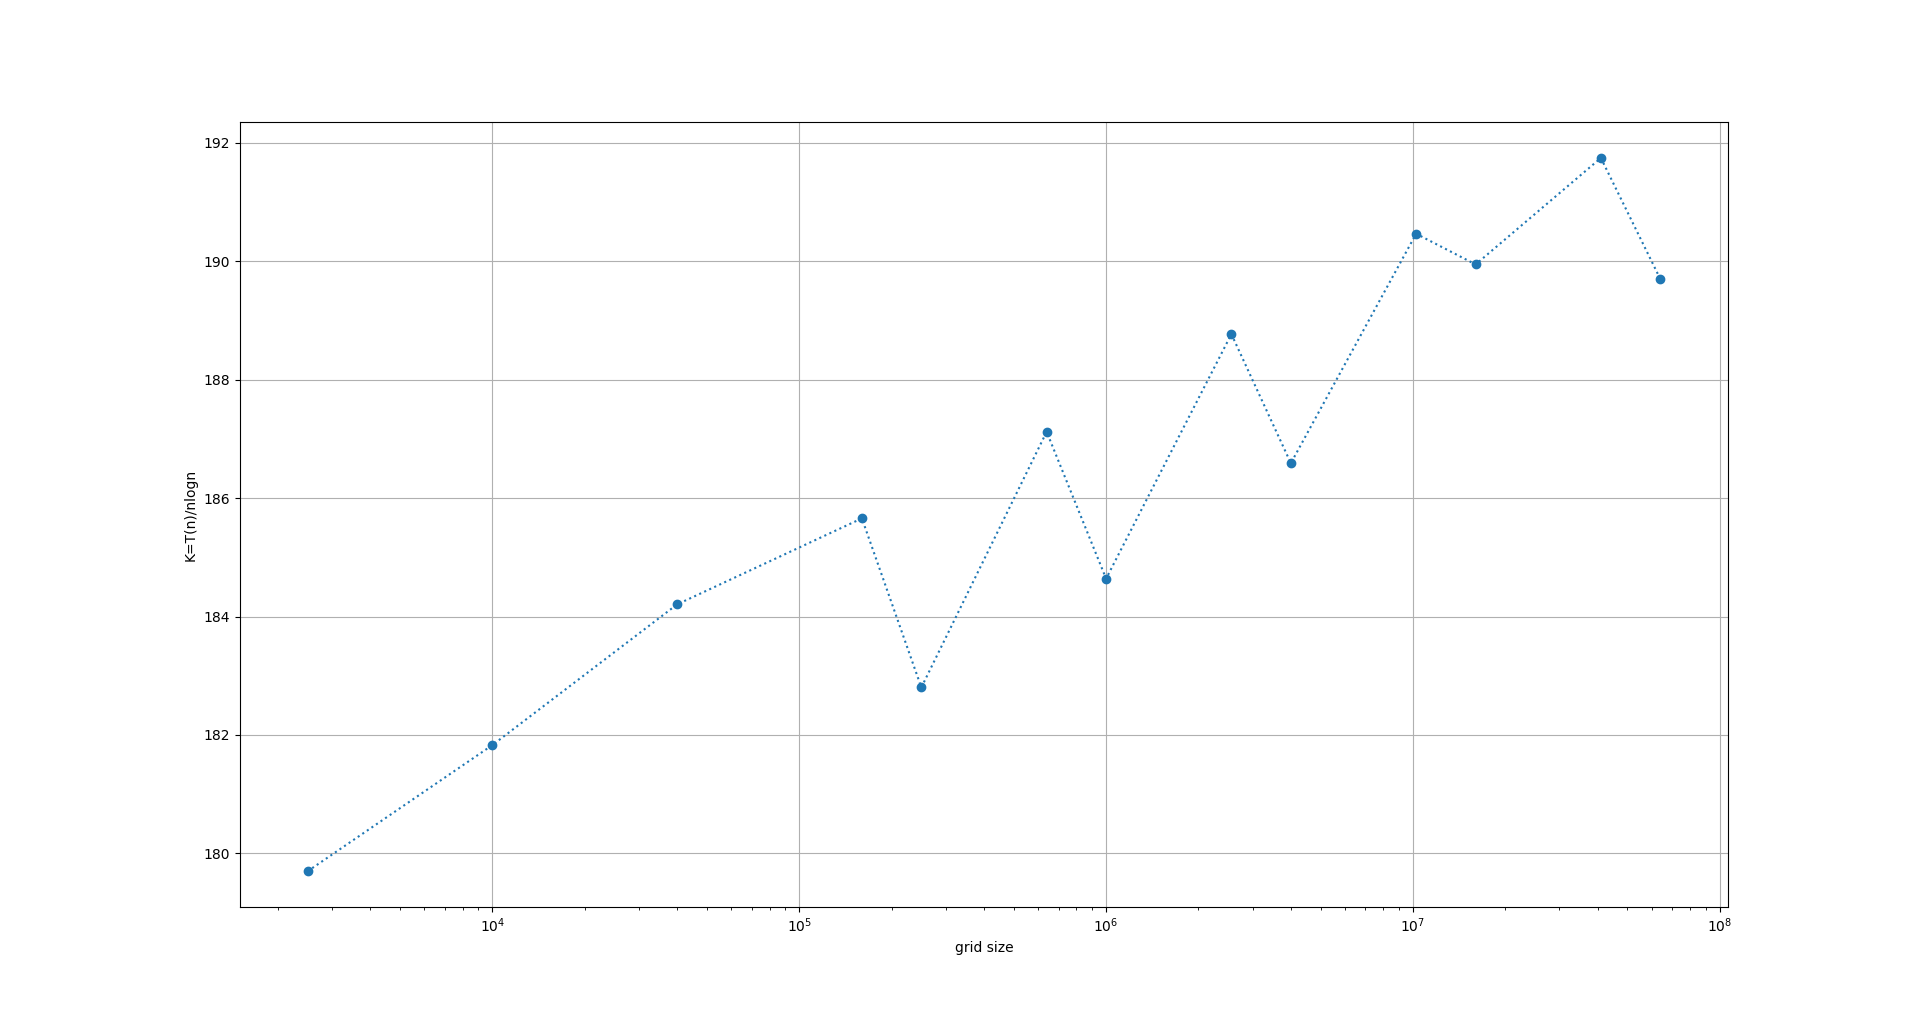
\includegraphics[scale=0.4]{constant}
	\caption{Константа алгоритма сортировки mergesort + insertion sort}
\end{figure}

Как видно, константа алгоритма изменяется незначительно при изменении размера входных данных в большом (достаточном для данной задачи) диапазоне. Определим относительный рост:
\begin{equation*}
\delta_K = \frac{K_{max}-K_{min}}{K_{min}} \cdot 100 \% = \frac{192-180}{180} \cdot 100 \% \approx 7 \%.
\end{equation*}

\begin{table}[H]
\centering
\begin{tabular}{ | c | c | }
	\hline
	$n$ & $K=10^9 \frac{T(n)} {n \log_2 n}$ \\
	\hline
	$2.5 \cdot 10^3$ & 180 \\
	$1.0 \cdot 10^4$ & 182 \\
	$4.0 \cdot 10^4$ & 186 \\
	$2.5 \cdot 10^5$ & 183 \\
	$6.4 \cdot 10^5$ & 187 \\
	$1.0 \cdot 10^6$ & 185 \\
	$2.5 \cdot 10^6$ & 189 \\
	$4.0 \cdot 10^6$ & 187 \\
	$1.0 \cdot 10^7$ & 190 \\
	$1.6 \cdot 10^7$ & 190 \\
	$4.1 \cdot 10^7$ & 192 \\
	$6.4 \cdot 10^7$ & 190 \\
	\hline
\end{tabular}
\end{table}

Для более точной оченки выполняемого времени константа алгоритма представлена ступенчатой функцией:
\[ K(n) = \begin{cases} 
      180 & n \leq 1.0 \cdot 10^4 \\
      185 & 1.0 \cdot 10^4 < x \leq 1.0 \cdot 10^6 \\
      190 & x > 1.0 \cdot 10^6
   \end{cases}
\]

\subsection{Параллельный алгоритм}
Как было сказано, для параллельной сортировки используется сеть обменной сортировки слиянием Бэтчера. Алгоритм построения сети, использованный в задании 1, был слегка изменён: теперь компараторы сети хранятся в массиве. Так как априори известно, что программа не будет запускаться на более чем 128 процессах, массив для хранения компараторов выделяется на стэке, позволяя хранить до 1471 компаратора.

\subsection{Запуск программы}
\begin{enumerate}
\item Если программа уже запущена, дождаться её завершения.
\item Указать необходимые параметры в файле makefile (размер сетки, число процессоров).
\item Создать и записать сетку в файл командой \text{make generate}.
\item Запустить сортировку командой \text{make sort\_par} (для однопроцессорной версии --- \text{make sort\_ser}). При запросе более 128 процессоров программа сообщит об ошибке во время работы. Аналогичное поведение будет в случае запроса двух и более процессоров при запуске последовательной версии программы.
\item Дождаться завершения.
\item При необходимости проверить правильность работы командой \text{make test}.
\item Результат одного запуска находится в папке ../out/ относительно файла makefile.
\end{enumerate}


\section{Используемая вычислительная система}
Результаты получены на суперкомпьютере Blue Gene/P. Эта машина имеет гибридную архитектуру: 2048 узлов, в пределах каждого из которых существуют 4 процессора с частотой 850 МГц (или ядра, поскольку они делят L3 кэш, имея собственные L1, L2 кэши) с общей оперативной памятью. Узлы соединены несколькими коммуникационными сетями: для коммуникаций точка-точка, для коллективных коммуникаций, для глобальных прерываний, для ввода-вывода, сеть управления (загрузка системы, отладка, мониторинг).  В данной задаче используются только взаимодействия точка-точка, поэтому целесообразно подробнее рассмотреть сеть трёхмерного тора. Сеть тора объединяет 2048 узлов (в максимальной конфигурации суперкомпьюетра она может объединять 73728 узлов), позволяя совмещать посылку данных и вычисления. Каждый узел в этой сети имеет 6 ближайших соседей (по два в каждом из трёх направлений), соседей соединяет пара кабелей --- один для чтения, другой для записи. Пропускная способность кабеля --- $425~ \text{МБ/с}$, суммарная пропускная способность узла --- $ 12 \cdot 425~ \text{МБ/с} = 5.1~ \text{ГБ/с}$ (см. ''IBM System Blue Gene Solution: Blue Gene/P Application Development'', издание 4). Латентность сети на уровне аппаратуры может достигать $5~\text{мкс}$, на уровне MPI --- $10~\text{мкс}$ (между самыми далёкими узлами; см. презентацию Федуловой И.A. ''Эффективное параллельное программирование с учетом особенностей IBM Blue Gene/P'' от 01.03.2010).

Ввиду архитектурных особенностей суперкомпьютера при использовании менее 512 узлов (в данной задаче не используется более 128 узлов) сеть тора недоступна: узлы объединяются в обычную трёхмерную решётку. Оценка латентности будет эвристической (см. след. раздел).

Существует три стратегии мэппинга процессов MPI на узлы Blue Gene/P: SMP (один узел --- один процесс), DUAL (до двух процессов на узле), VN (до четырёх процессов на узле). В данной работе используется режим SMP, причём нити не порождаются внутри узлов. Этот режим работает быстрее DUAL и VN, так как процессы не делят между собой коммутатор узла. С другой стороны, эффективность использования суперкомпьютера очень низка --- на каждом узле работает только 1 из 4 процессоров.

\section{Анализ времени выполнения сортировки Бэтчера}
Число тактов, затрачиваемых сортировкой Бэтчера, можно получить аналитически для случаев, когда число процессоров является степенью двойки. Для асимптотического анализа алгоритма этого достаточно.

Обозначим $B(p)$ --- число тактов, требуемое сортировке на $p$ процессорах, $S(p)$ --- число тактов, требуемое для операции слияния на $p$ процессорах, когда обе половины массива элементов отсортированы.

\begin{figure}[H]
	\centering
	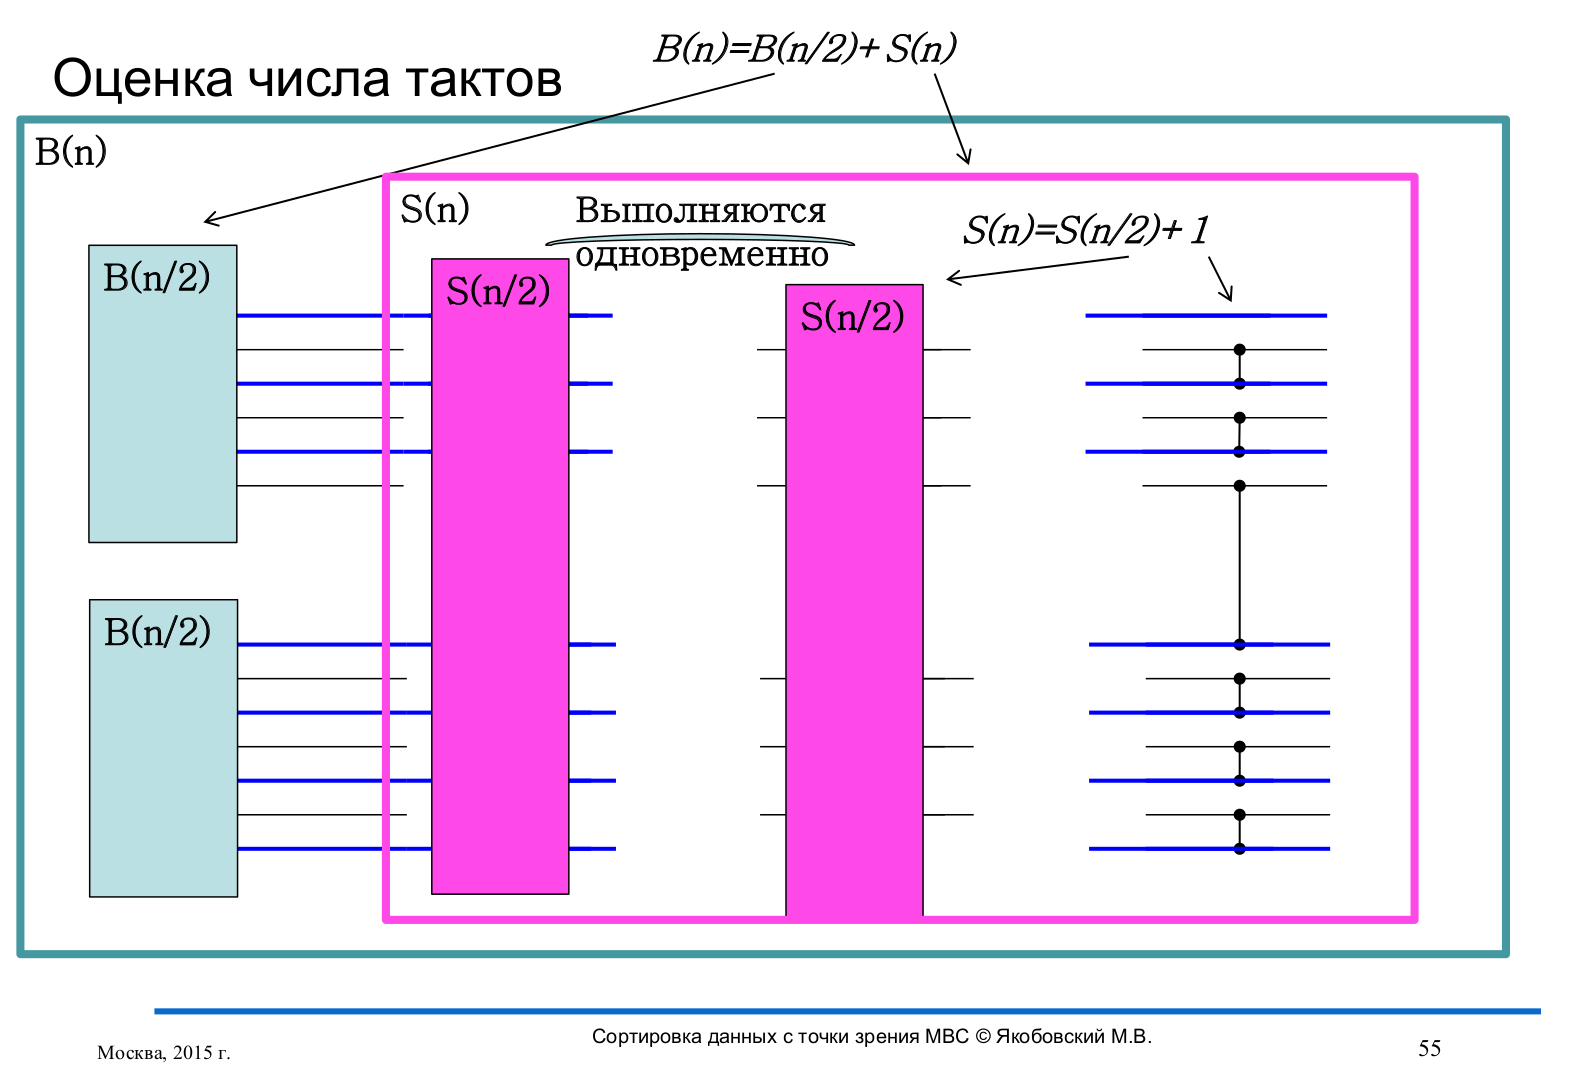
\includegraphics[scale=0.4]{tacts}
\end{figure}

Получим систему уравнений:
\begin{equation*}
B(p) = B \left( \frac{p}{2} \right) + S(p)
\end{equation*}
\begin{equation*}
S(p) = S \left( \frac{p}{2} \right) + 1.
\end{equation*}

Зная, что $B(2) = 1$, $S(2) = 1$, получим выражения, определяющие задержку сети:
\begin{equation*}
S(p) = \log_2 p
\end{equation*}
\begin{equation*}
B(p) = \frac{\log_2 p \left( \log_2 p + 1 \right)}{2}
\end{equation*}

Каждый такт --- это пересылка $\frac{n}{p}$ элементов между процессорами и слияние двух последовательностей из $\frac{n}{p}$ элементов в две последовательности того же размера, причём процесс с меньшим рангом собирает меньшие элементы. Считая, что пересылка данных между двумя процессорами не зависит от загруженности сети и время передачи $n$ байт описывается формулой
$$ t(n) = L + n \tau_s, $$
где $L$ --- латентность сети, $\tau_s$ --- время пересылки одного байта, для времени одного такта получим (передача и приём сообщения происходят независимо):
$$ T_{join} = L + \frac{n}{p} s_0 \tau_s + \alpha \frac{n}{p}.$$
Здесь $s_0$ --- размер одного элемента в байтах. Учитывая, что время выполнения последовательной сортировки равно
$$K \frac{n}{p} \log_2 \frac{n}{p},$$
получим полное время работы сортировки:
\begin{equation*}
T_p(n) = \frac{n}{p} \left( K \log_2 \frac{n}{p} + (\alpha + s_0\tau_s) \frac{\log_2 p (\log_2 p + 1)}{2} \right) + L \frac{\log_2 p (\log_2 p + 1)}{2}.
\end{equation*}
Будем считать, что константы последовательной сортировки (основанной на слиянии) и собственно слияния равны: $ K = \alpha $.
Тогда мы имеем все необходимые для расчёта величины: коэффициент $K$ задан таблично, $s_0 = 12 ~ \text{байт}$, $\tau_s = \frac{1}{bandwidth} = \frac{1}{425 \cdot 1024 \cdot 1024} \approx 2.2 ~ \text{нс/байт}$, для оценки латентности взято число $L = 0.1 ~ \text{мс}$ (которое, впрочем, в 100 раз меньше заявленного максимума; можно даже взять ноль --- радикальных отличий от выбранного значения не будет).

Рассмотрим случай мгновенных пересылок для указания верхней границы эффективности алгоритма: $ \tau_s = 0 $, $ L = 0 $. Тогда время сортировки $n$ элементов на $p$ процессорах будет следующим:
\begin{equation*}
T_p(n) = K \frac{n}{p} \left( \log_2 \frac{n}{p} + \frac{\log_2 p (\log_2 p + 1)}{2} \right).
\end{equation*}

Лучший последовательный алгоритм срабатывает за время
$$ T_1(n) = K n \log_2 n.$$
Ускорение и эффективность алгоритма:
\begin{equation*}
S_p(n) = \frac{T_1(n)}{T_p(n)} = p \frac{1}{1 - \log_n p + \frac{\log_2 p (\log_2 p + 1)}{2 \log_2 n}},
\end{equation*}
\begin{equation*}
E_p(n) = \frac{T_1(n)}{pT_p(n)} = \frac{1}{1 - \log_n p + \frac{\log_2 p (\log_2 p + 1)}{2 \log_2 n}}.
\end{equation*}
Например, для $p=128$, $n=6,4 \cdot 10^7$ максимально достижимая эффективность равна 55\%.

\section{Результаты}
На приведённых ниже графиках изображены только реальные данные, полученные на суперкомпьютере. Видно, что при небольшом числе процессоров задача масштабируется одинаково для разных размеров сетки. Существенные различия в ускорении появляются при наличии 64 и более процессоров: чем больше размер сетки, тем выше ускорение. Очевидно, коммуникационные издержки играют меньшую роль при большем времени автономной работы каждого процессора.

Эффективность свыше 50\% на 128 процессорах удалось достичь при размере сетки $8000 \times 8000$. 

Интересно заметить, что на двух процессорах при размере сетки $4000 \times 4000$ было получено незначительное сверхлинейное ускорение.

\begin{figure}[H]
	\centering
	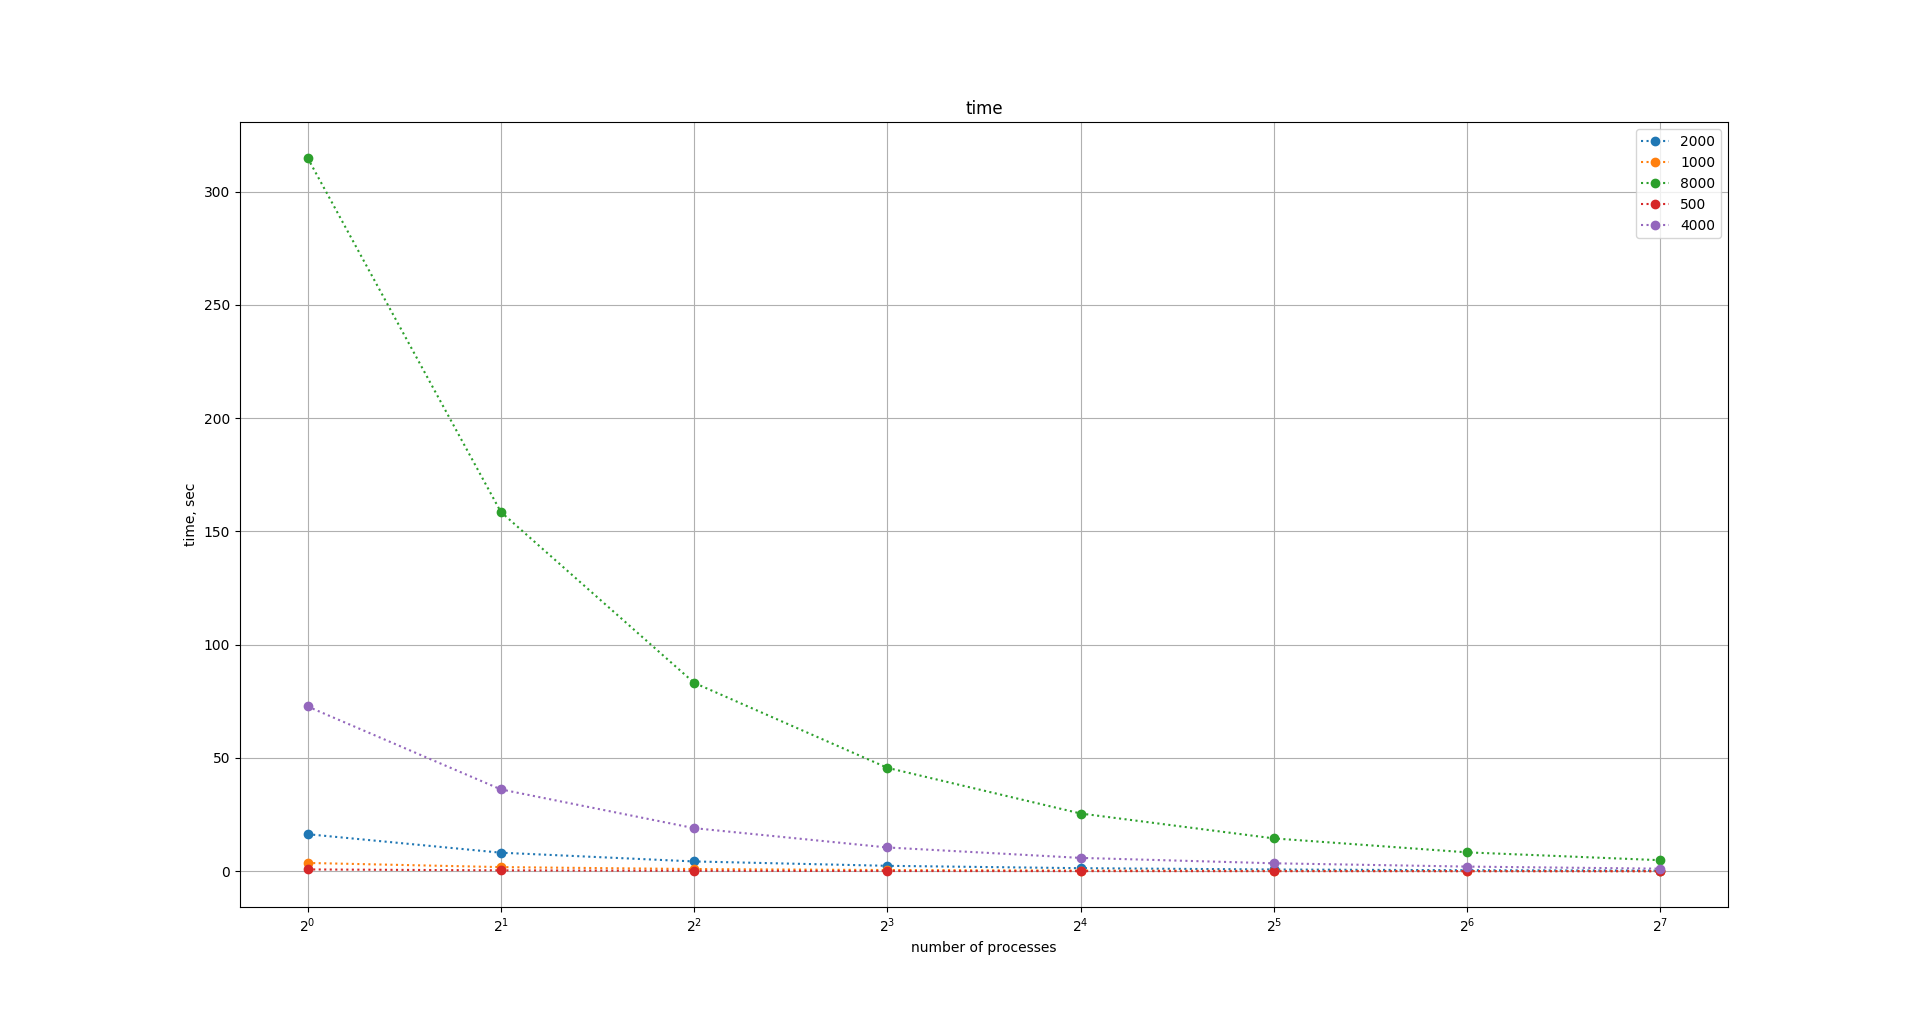
\includegraphics[scale=0.4]{time}
\end{figure}

\begin{figure}[H]
	\centering
	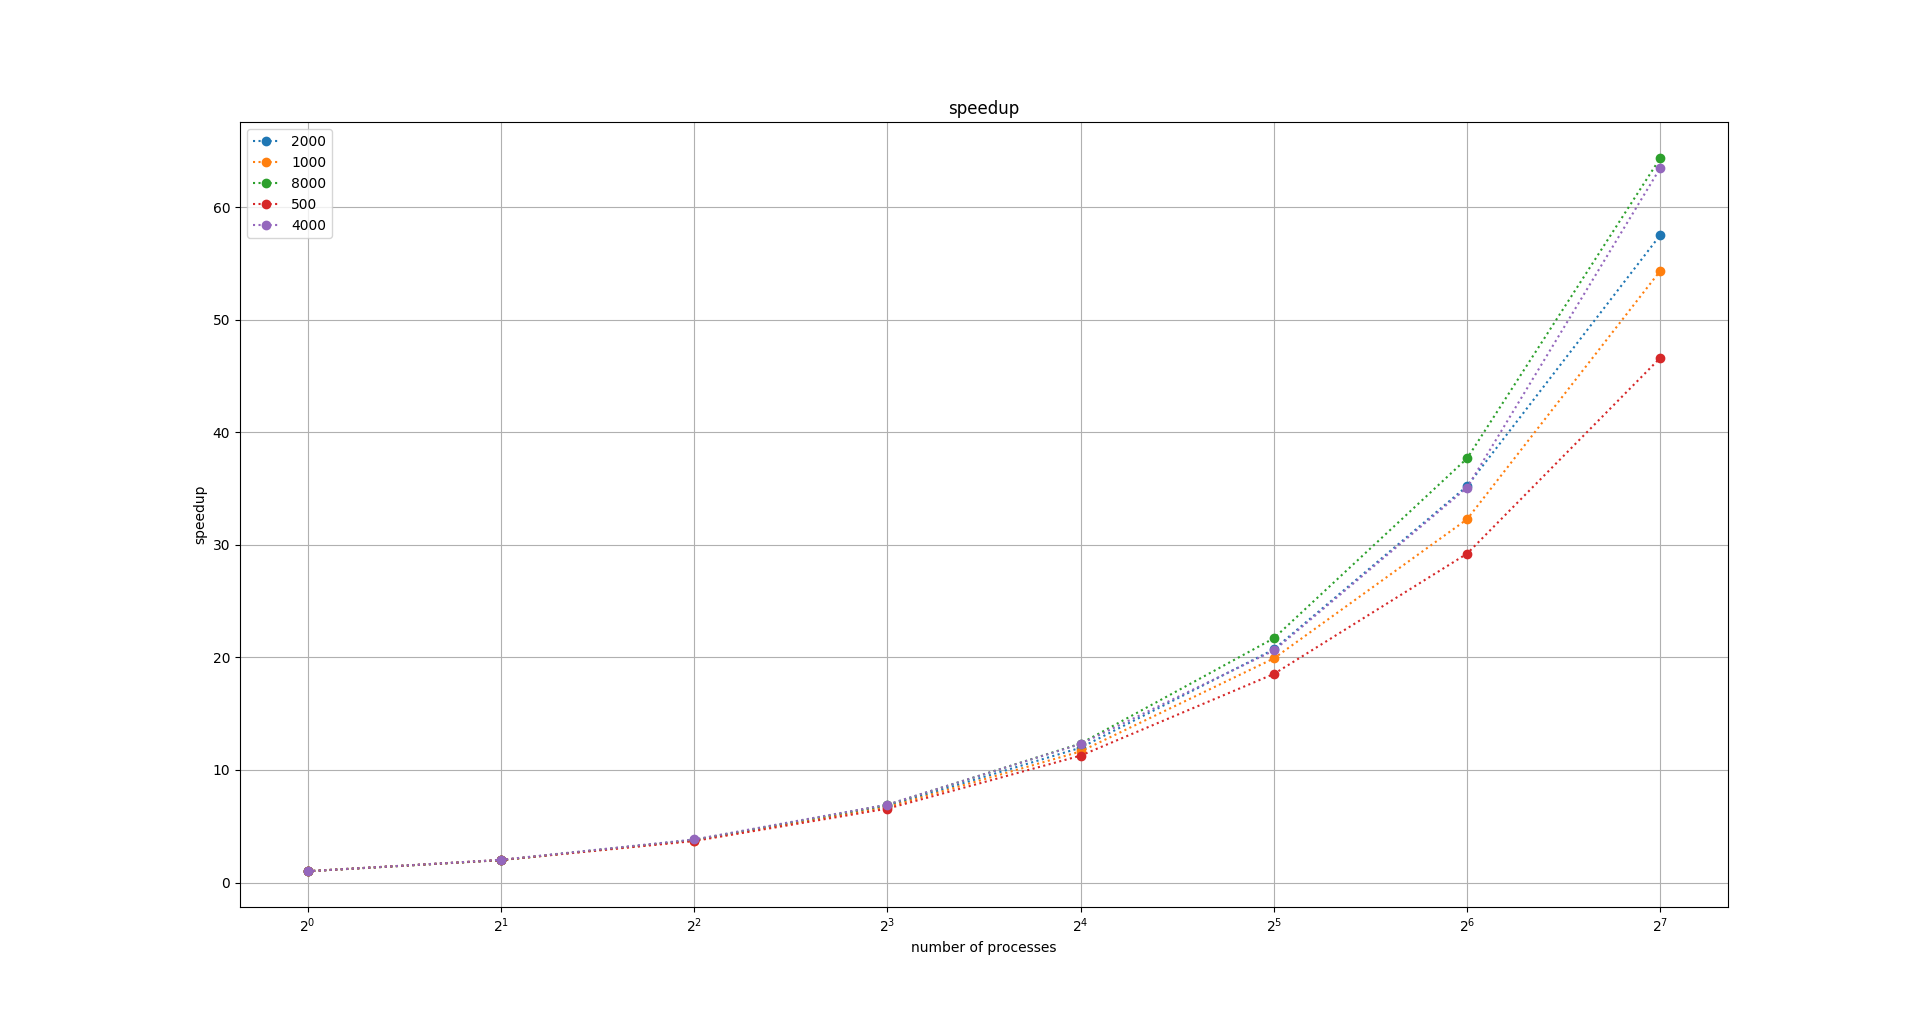
\includegraphics[scale=0.4]{speedup}
\end{figure}

\begin{figure}[H]
	\centering
	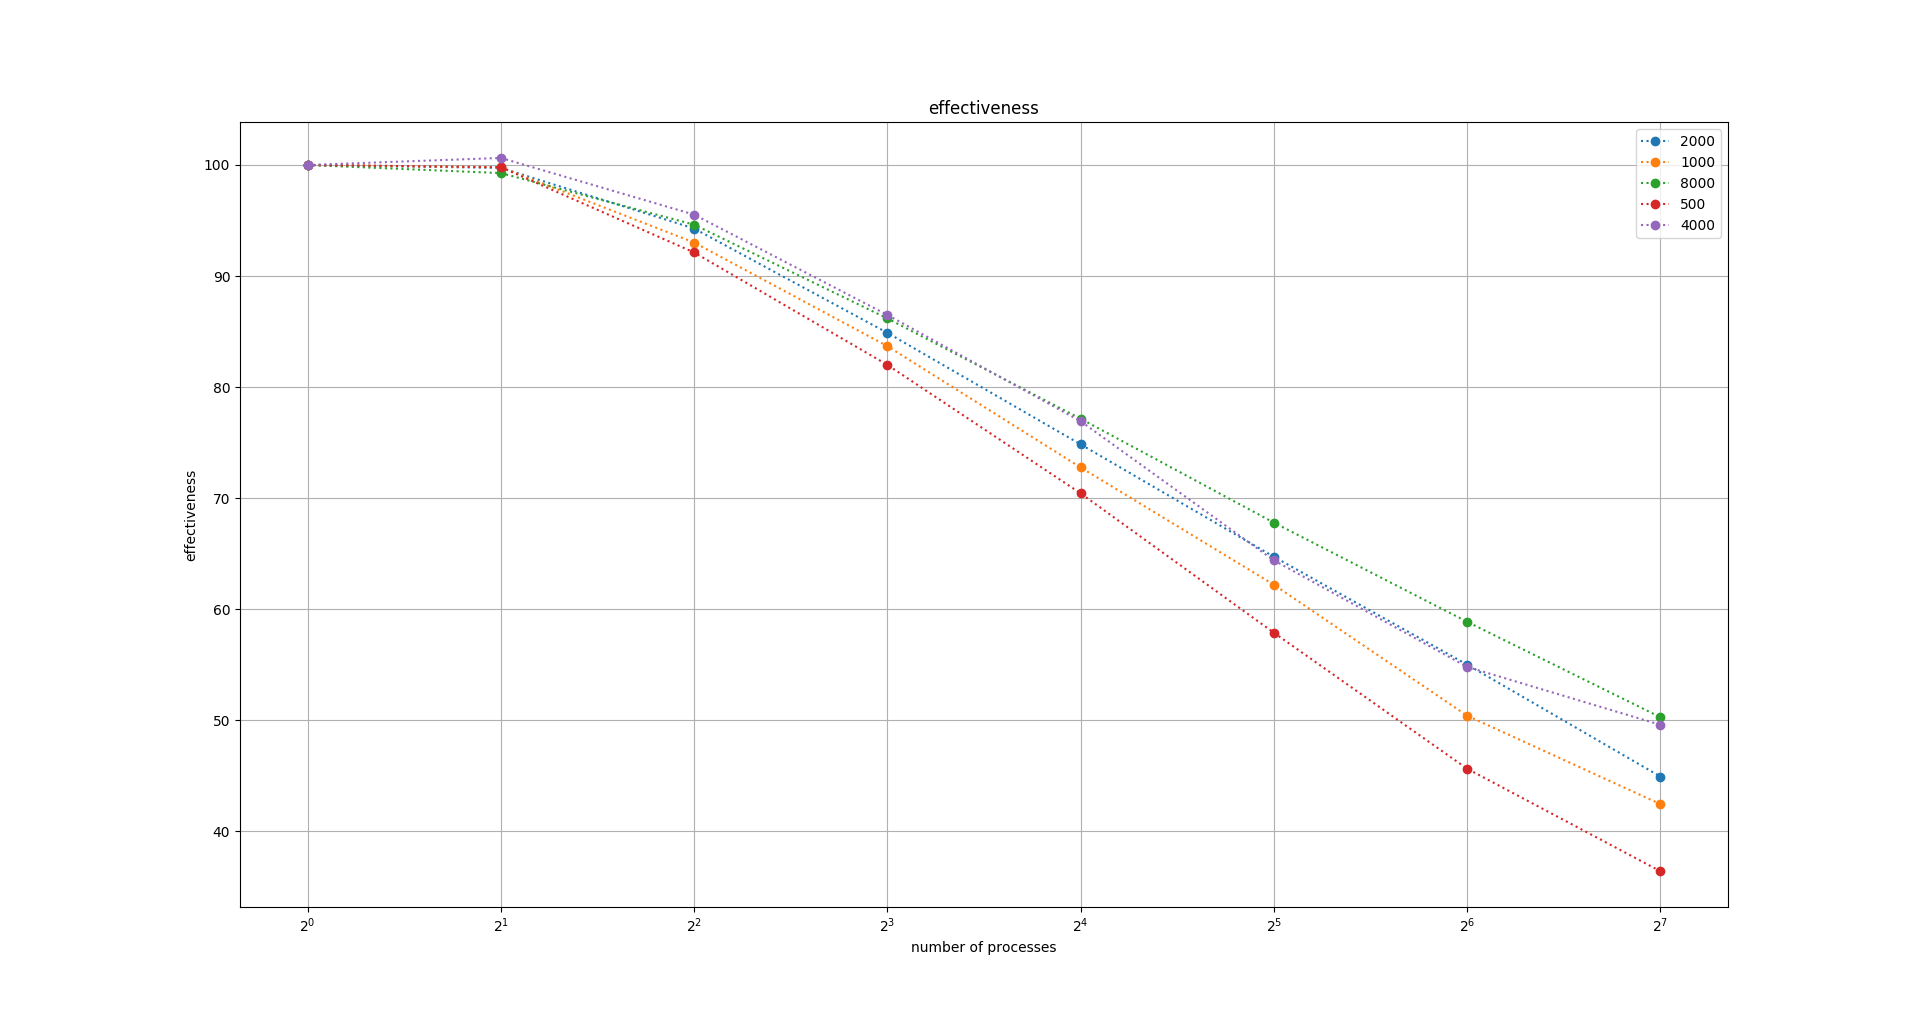
\includegraphics[scale=0.4]{effectiveness}
\end{figure}

В таблицах реальные данные обозначаются буквами $T, S, E$, оценочные --- $\hat T, \hat S, \hat E$. Очевидно, можно утверждать, что программная реализация согласуется с описанным выше алгоритмом сортировки. Наибольшие расхождения теоретических и практических времён составляют $ \approx 5.7 \% $ (сетка $4000 \times 4000$, 32 процессора), тогда как среднее расхождение не превышает $ 3 \% $. Видимо, этот пик в $5.7 \%$ можно было бы избежать, если бы время реальное сортировки усреднялось по нескольким запускам программы.

\begin{table}[H]
\centering
\begin{tabular}{ | c | c | c | c | c | c | c | c | c | }
	\hline
	\multicolumn{9}{ | c | }{$500 \times 500$} \\
	\hline
	nodes & cores & $T_p,sec$ & $S(p)$ & $E(p)$ & tacts & $\hat T_p(n),sec$ & $\hat S_p(n)$ & $\hat E_p(n)$ \\
	\hline
	1   & 1   & 0.819 & 1.00 & 100.0 & 0  & 0.83  & 1.00 & 100.0 \\
	2   & 2   & 0.411 & 2.00 & 99.8  & 1  & 0.42  & 1.98 & 99.2  \\
	4   & 4   & 0.222 & 3.68 & 92.1  & 3  & 0.22  & 3.70 & 92.5  \\
	8   & 8   & 0.125 & 6.56 & 82.0  & 6  & 0.126 & 6.55 & 81.8  \\
	16  & 16  & 0.072 & 11.3 & 70.4  & 10 & 0.074 & 11.1 & 69.7  \\
	32  & 32  & 0.044 & 18.5 & 57.9  & 15 & 0.044 & 18.9 & 59.0  \\
	64  & 64  & 0.028 & 29.2 & 45.6  & 21 & 0.027 & 30.2 & 47.2  \\
	128 & 128 & 0.018 & 46.6 & 36.4  & 28 & 0.018 & 46.2 & 36.1  \\
	\hline
\end{tabular}
\end{table}

\begin{table}[H]
\centering
\begin{tabular}{ | c | c | c | c | c | c | c | c | c | }
	\hline
	\multicolumn{9}{ | c | }{$1000 \times 1000$} \\
	\hline
	nodes & cores & $T_p,sec$ & $S(p)$ & $E(p)$ & tacts & $\hat T_p(n),sec$ & $\hat S_p(n)$ & $\hat E_p(n)$ \\
	\hline
	1   & 1   & 3.680 & 1.00 & 100.0 & 0  & 3.69  & 1.00 & 100.0 \\
	2   & 2   & 1.844 & 2.00 & 99.8  & 1  & 1.86  & 1.99 & 99.3  \\
	4   & 4   & 0.989 & 3.72 & 93.0  & 3  & 0.989 & 3.73 & 93.2  \\
	8   & 8   & 0.550 & 6.70 & 83.7  & 6  & 0.551 & 6.69 & 83.6  \\
	16  & 16  & 0.316 & 11.6 & 72.8  & 10 & 0.318 & 11.6 & 72.5  \\
	32  & 32  & 0.185 & 19.9 & 62.2  & 15 & 0.187 & 19.7 & 61.6  \\
	64  & 64  & 0.114 & 32.3 & 50.4  & 21 & 0.112 & 32.9 & 51.5  \\
	128 & 128 & 0.068 & 54.4 & 42.5  & 28 & 0.066 & 55.7 & 43.5  \\
	\hline
\end{tabular}
\end{table}

\begin{table}[H]
\centering
\begin{tabular}{ | c | c | c | c | c | c | c | c | c | }
	\hline
	\multicolumn{9}{ | c | }{$2000 \times 2000$} \\
	\hline
	nodes & cores & $T_p,sec$ & $S(p)$ & $E(p)$ & tacts & $\hat T_p(n),sec$ & $\hat S_p(n)$ & $\hat E_p(n)$ \\
	\hline
	1   & 1   & 16.37 & 1.00 & 100.0 & 0  & 16.7 & 1.00 & 100.0 \\
	2   & 2   & 8.20  & 1.99 & 99.7  & 1  & 8.39 & 1.99 & 99.4  \\
	4   & 4   & 4.34  & 3.77 & 94.3  & 3  & 4.32 & 3.86 & 96.4  \\
	8   & 8   & 2.41  & 6.79 & 84.9  & 6  & 2.39 & 6.98 & 87.3  \\
	16  & 16  & 1.37  & 12.0 & 74.8  & 10 & 1.36 & 12.3 & 76.6  \\
	32  & 32  & 0.79  & 20.7 & 64.7  & 15 & 0.79 & 21.1 & 65.9  \\
	64  & 64  & 0.46  & 35.2 & 55.0  & 21 & 0.46 & 35.9 & 56.1  \\
	128 & 128 & 0.28  & 57.5 & 44.9  & 28 & 0.27 & 60.1 & 47.4  \\
	\hline
\end{tabular}
\end{table}

\begin{table}[H]
\centering
\begin{tabular}{ | c | c | c | c | c | c | c | c | c | }
	\hline
	\multicolumn{9}{ | c | }{$4000 \times 4000$} \\
	\hline
	nodes & cores & $T_p,sec$ & $S(p)$ & $E(p)$ & tacts & $\hat T_p(n),sec$ & $\hat S_p(n)$ & $\hat E_p(n)$ \\
	\hline
	1   & 1   & 72.7  & 1.00 & 100.0 & 0  & 72.8 & 1.00 & 100.0 \\
	2   & 2   & 36.1  & 2.01 & 100.6 & 1  & 36.6 & 1.99 & 99.4  \\
	4   & 4   & 19.0  & 3.82 & 95.5  & 3  & 19.3 & 3.78 & 94.4  \\
	8   & 8   & 10.5  & 6.89 & 86.5  & 6  & 10.6 & 6.89 & 86.1  \\
	16  & 16  & 5.91  & 12.3 & 76.9  & 10 & 5.81 & 12.5 & 78.3  \\
	32  & 32  & 3.53  & 20.6 & 64.4  & 15 & 3.34 & 21.8 & 68.0  \\
	64  & 64  & 2.07  & 35.1 & 54.8  & 21 & 1.94 & 37.4 & 58.5  \\
	128 & 128 & 1.15  & 63.5 & 49.6  & 28 & 1.14 & 64.0 & 50.0  \\
	\hline
\end{tabular}
\end{table}

\begin{table}[H]
\centering
\begin{tabular}{ | c | c | c | c | c | c | c | c | c | }
	\hline
	\multicolumn{9}{ | c | }{$8000 \times 8000$} \\
	\hline
	nodes & cores & $T_p,sec$ & $S(p)$ & $E(p)$ & tacts & $\hat T_p(n),sec$ & $\hat S_p(n)$ & $\hat E_p(n)$ \\
	\hline
	1   & 1   & 315   & 1.00 & 100.0 & 0  & 315  & 1.00 & 100.0 \\
	2   & 2   & 159   & 1.99 & 99.3  & 1  & 159  & 1.99 & 99.5  \\
	4   & 4   & 83.2  & 3.79 & 94.6  & 3  & 83.2 & 3.79 & 94.8  \\
	8   & 8   & 45.7  & 6.89 & 86.2  & 6  & 45.3 & 6.97 & 87.1  \\
	16  & 16  & 25.5  & 12.3 & 77.2  & 10 & 25.3 & 12.4 & 77.8  \\
	32  & 32  & 14.5  & 21.7 & 67.8  & 15 & 14.5 & 21.8 & 68.1  \\
	64  & 64  & 8.36  & 37.7 & 58.9  & 21 & 8.14 & 38.7 & 60.5  \\
	128 & 128 & 4.89  & 64.4 & 50.3  & 28 & 4.72 & 66.8 & 52.2  \\
	\hline
\end{tabular}
\end{table}


\end{document}\grid
